\documentclass{beamer}

\usetheme{Warsaw}
\usepackage[utf8]{inputenc}
\usepackage{tikz}
\usepackage{bm}
\usepackage{pgfplots}
\usepackage{graphicx}
\usepackage{gensymb}
\usepackage{sidecap}
\usepackage{wasysym}
\usepackage{fancybox}

\pgfplotsset{compat=1.4}
\usepgfplotslibrary{units}

\setbeamertemplate{footline}[frame number]
\setbeamertemplate{frametitle}[default][center]

\mode<presentation>{
	\usetheme{Warsaw}
	%\setbeamercovered{transparent}
	\usecolortheme{seagull}
}

\setbeamertemplate{headline}{}

\definecolor{pemblue}{RGB}{1,123,165}
\setbeamercolor*{palette primary}{fg=black,bg=pemblue!80}
\setbeamercolor*{palette secondary}{fg=black,bg=pemblue!80!gray!80}
\setbeamercolor*{palette tertiary}{fg=black,bg=pemblue!100}
\setbeamercolor*{palette quaternary}{fg=black,bg=pemblue!110}

\uselanguage{portuguese}
\languagepath{portuguese}
\deftranslation[to=portuguese]{Definition}{Definição}
\deftranslation[to=portuguese]{Corollary}{Identidades}

\usebackgroundtemplate
{%
	\begin{picture}(210,40)(-5,2)
	\includegraphics[width=0.07\paperwidth,keepaspectratio]{imgs/pem-logo-short.png}
	\end{picture}%
}

\title{Estimativa
	de condutâncias térmicas de contato em interfaces irregulares usando a
	técnica da Transformada Integral Clássica e o método dos funcionais de reciprocidade}
\author{Guilherme Camelo de Freitas}
\date{28 de Junho de 2019}

\institute
{
	Universidade Federal do Rio de Janeiro\\
	UFRJ/COPPE/PEM
}

\newcommand{\graficostemperatura}[5]{%
	\begin{minipage}[t][6cm][c]{4.5cm}
		\centering		
		\begin{tikzpicture}[scale=0.75]
		\begin{axis}[
		%/pgf/number format/1000 sep={.},/pgf/number format/use comma,
		axis lines=left,
		%		xmin = 0,
		%		xmax = 0.04,
		%ymin = #4,
		%ymax = #5,
		%		restrict y to domain=-500:2000,
		scaled x ticks = false,
		scaled y ticks = false,
		x tick label style={/pgf/number format/fixed},
		y tick label style={/pgf/number format/fixed},
		anchor=east,  
		width=7cm,
		height=5cm,
		label style={font=\footnotesize},
		xlabel = $x$(m),
		ylabel= $T_1\big|_{\Gamma_0}$ (\celsius),
		ylabel style={rotate=-90, at={(-0.1, 1)}, anchor = south west}]		
		\pgfplotstableread{../data/temperaturas_sinteticas_interface_0#1_conductance_0#2_stdev_05.dat} 
		\teff
		\addplot[only marks,color=gray,mark=triangle,mark options={mark size=2.0pt}] table from \teff;
		\pgfplotstableread{../data/temperaturas_sinteticas_interface_0#1_conductance_0#2_stdev_01.dat} 
		\teff
		\addplot[only marks,color=red,mark=square,mark options={mark size=2.0pt}] table from \teff;
		\pgfplotstableread{../data/temperaturas_sinteticas_interface_0#1_conductance_0#2_stdev_00.dat} 
		\teff
		\addplot[color=blue,mark=o,mark options={mark size=2.0pt}] table from \teff;		
		\end{axis}
		\end{tikzpicture}
		\caption*{(#3) Perfil #2}
	\end{minipage}
}%

% Parametros:
% erro_rms
% delta_temperatura ou fluxo_calor
% interface_id: 1, 2, ou 3
% condutance_id: 1, 2, ou 3
% axis text
% a, b, ou c
\newcommand{\graficoerrorms}[6]{%
	\begin{minipage}[t][6cm][c]{4.5cm}
		\centering		
		\begin{tikzpicture}[scale=0.75]
		\begin{axis}[
		axis lines=left,
		%/pgf/number format/1000 sep={.},/pgf/number format/use comma,
		%ymode = log,
		grid=major,
		legend style={legend pos=north west}
		% xmin = 0.00000001,
		%		xmax = 0.04,
		%ymin = 0,
		%ymax = 90,
		scaled x ticks = true,
		scaled y ticks = true,
		x tick label style={/pgf/number format/fixed},
		y tick label style={/pgf/number format/fixed},
		xtick = {0,5,10,15,20,25,30,35,40,45,50},
		anchor=east,  
		width=7cm,
		height=6cm,
		label style={font=\footnotesize},
		xlabel = $N_j$,
		ylabel= $\log\left(\delta_{#5}\right)$,
		ylabel style={rotate=-90, at={(-0.1, 1)}, anchor = south west}]
		\pgfplotstableread{../data/#1_#2_interface_0#3_conductance_0#4_stdev_00.dat} 
		\teff
		\addplot[color=blue,mark=o,mark options={mark size=2.0pt}] table from \teff;
		\pgfplotstableread{../data/#1_#2_interface_0#3_conductance_0#4_stdev_01.dat} 
		\teff
		\addplot[color=red,mark=square,mark options={mark size=2.0pt}] table from \teff;
		\pgfplotstableread{../data/#1_#2_interface_0#3_conductance_0#4_stdev_05.dat} 
		\teff
		\addplot[color=gray,mark=triangle,mark options={mark size=2.0pt}] table from \teff;
		\end{axis}
		\end{tikzpicture}
		\caption*{(#6)Perfil #4}
	\end{minipage}
}%

%Parametros
% delta_temperatura ou fluxo_calor
% interface_idx : 1, 2, ou 3
% condutance_idx : 1, 2, ou 3
% numero de autofunces para cada desvio padrao, com dois algarismos
% a, b, ou c
\newcommand{\graficoestimativa}[9]{%
	\begin{minipage}[c][3cm][c]{0.3\textwidth}
		\centering		
		\begin{tikzpicture}[scale=0.65]
		\begin{axis}[
		axis lines=left,
		%/pgf/number format/1000 sep={.},/pgf/number format/use comma,
		%		xmin = 0,
		%		xmax = 0.04,
		%		ymin = 310,
		%		ymax = 340,
		%		restrict y to domain=-500:2000,
		scaled x ticks = false,
		scaled y ticks = false,
		x tick label style={/pgf/number format/fixed},
		y tick label style={/pgf/number format/fixed},
		anchor=east,  
		width=5cm,
		height=4cm,
		label style={font=\footnotesize},
		xlabel = $x$(m),
		ylabel= $#8$ (#9),
		ylabel style={rotate=-90, at={(-0.1, 1)}, anchor = south west}]
		\pgfplotstableread{../data/comsol/#1_interface_0#2_conductance_0#3.dat} 
		\teff
		\addplot[color=black, line width=1.5pt] table from \teff;
		\pgfplotstableread{../data/fortran/#1_interface_0#2_conductance_0#3_stdev_00_N_#4.dat} 
		\teff
		\addplot[only marks, color=blue,mark=o,mark options={mark size=1.5pt}] table from \teff;
		\pgfplotstableread{../data/fortran/#1_interface_0#2_conductance_0#3_stdev_01_N_#5.dat} 
		\teff
		\addplot[only marks,color=red,mark=square,mark options={mark size=1.5pt}] table from \teff;
		\pgfplotstableread{../data/fortran/#1_interface_0#2_conductance_0#3_stdev_05_N_#6.dat} 
		\teff
		\addplot[only marks,color=gray,mark=triangle,mark options={mark size=1.5pt}] table from \teff;
		\end{axis}
		\end{tikzpicture}
		%\caption*{(#7) Perfil #3}
	\end{minipage}
}%

\newcommand{\graficoctc}[4]{%
	\begin{minipage}[t][3cm][c]{0.3\textwidth}
		\centering		
		\begin{tikzpicture}[scale=0.65]
		\begin{axis}[
		axis lines=left,
		%/pgf/number format/1000 sep={.},/pgf/number format/use comma,
		%		xmin = 0,
		%		xmax = 0.04,
		%		ymin = 310,
		%		ymax = 340,
		%		restrict y to domain=-500:2000,
		scaled x ticks = false,
		scaled y ticks = false,
		x tick label style={/pgf/number format/fixed},
		y tick label style={/pgf/number format/fixed},
		anchor=east,  
		width=5cm,
		height=4cm,
		label style={font=\footnotesize},
		xlabel = $x$(m),
		ylabel= $h_c$ (W/$\text{m}^2$\celsius),
		ylabel style={rotate=-90, at={(-0.1, 1)}, anchor = south west}]
		\pgfplotstableread{../data/conductance_#2.dat} 
		\teff
		\addplot[color=black, line width=1.5pt] table from \teff;
		\pgfplotstableread{../data/estimativa_ctc_interface_#1_conductance_#2_stdev_00.dat} 
		\teff
		\addplot[only marks, color=blue,mark=o,mark options={mark size=1.5pt}] table from \teff;
		\pgfplotstableread{../data/estimativa_ctc_interface_#1_conductance_#2_stdev_01.dat} 
		\teff
		\addplot[only marks,color=red,mark=square,mark options={mark size=1.5pt}] table from \teff;
		\pgfplotstableread{../data/estimativa_ctc_interface_#1_conductance_#2_stdev_05.dat} 
		\teff
		\addplot[only marks,color=gray,mark=triangle,mark options={mark size=1.5pt}] table from \teff;
		\end{axis}
		\end{tikzpicture}
		%\caption*{(#4) Perfil #3}
	\end{minipage}
}%

\newcommand{\graficosmetricas}[4]{%
	\begin{minipage}[t][6cm][c]{4.5cm}
	\centering		
	\begin{tikzpicture}[scale=0.75]
	\begin{axis}[
	%/pgf/number format/1000 sep={.},/pgf/number format/use comma,
	axis lines=left,
	ymode = log,
	scaled x ticks = false,
	scaled y ticks = false,
	x tick label style={/pgf/number format/fixed},
	y tick label style={/pgf/number format/fixed},
	anchor=east,  
	width=7cm,
	height=5cm,
	label style={font=\footnotesize},
	xlabel = $x$(m),
	ylabel= $T_1\big|_{\Gamma_0}$ (\celsius),
	ylabel style={rotate=-90, at={(-0.1, 1)}, anchor = south west}]			
	\addplot[color=blue,mark=triangle,mark options={mark size=2.0pt}] table[x index=0,y index=#4] {../data/erro_rms_interface_0#1_conductance_0#2_stdev_0#3.dat};				
	\end{axis}
	\end{tikzpicture}
	%\caption*{(#3) Perfil #2}
	\end{minipage}
}%

\newcommand{\graficointerface}[1]{%
	\begin{minipage}[c][2cm][c]{\textwidth}
	\centering
	\begin{tikzpicture}[scale=0.5]
	\begin{axis}[
	anchor=east,  
	ticks=none,
	width=6cm,
	height=3cm,
	%ylabel=Iterações Lineares,
	xmin = 0,
	xmax = 0.04,
	ymin = 0,
	ymax = 0.02]
	\pgfplotstableread{../data/interface_0#1.dat} 
	\teff
	\addplot[color=blue,mark=none,smooth] table from \teff;
	\end{axis}			
	\end{tikzpicture}	
	\end{minipage}
}%

\newcommand{\graficosctclegenda}{%
	\begin{minipage}[c][2cm][c]{0.3\textwidth}
	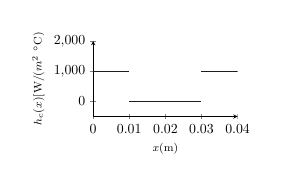
\begin{tikzpicture}[scale=0.5]
	\begin{axis}[
	%/pgf/number format/1000 sep={.},/pgf/number format/use comma,
	axis lines=left,
	xmin = 0,
	xmax = 0.04,
	ymin = -500,
	ymax = 2000,
	restrict y to domain=-500:2000,
	scaled x ticks = false,
	scaled y ticks = false,
	x tick label style={/pgf/number format/fixed},
	y tick label style={/pgf/number format/fixed},
	anchor=east,  
	width=5.25cm,
	height=3.5cm,
	label style={font=\footnotesize},
	xlabel = $x$(m),
	ylabel= $h_c(x)[$W/($\text{m}^2$ \celsius)]]
	\addplot[color=blue,mark=none,smooth, domain=0:0.01] {1000};
	\addplot[color=blue,mark=none,smooth, domain=0.01:0.03] {0};
	\addplot[color=blue,mark=none,smooth, domain=0.03:0.04] {1000};
	\end{axis}			
	\end{tikzpicture}	
	\end{minipage}
	\begin{minipage}[c][2cm][c]{0.3\textwidth}
	\begin{tikzpicture}[scale=0.5]
	\begin{axis}[
	%/pgf/number format/1000 sep={.},/pgf/number format/use comma,
	axis lines=left,
	xmin = 0,
	xmax = 0.04,
	ymin = -500,
	ymax = 2000,
	restrict y to domain=-500:2000,
	scaled x ticks = false,
	scaled y ticks = false,
	x tick label style={/pgf/number format/fixed},
	y tick label style={/pgf/number format/fixed},
	anchor=east,  
	width=5.25cm,
	height=3.5cm,
	label style={font=\footnotesize},
	xlabel = $x$(m),
	ylabel= $h_c(x)$[W/($\text{m}^2$ \celsius)]]
	\pgfplotstableread{../data/conductance_02.dat} 
	\teff
	\addplot[color=blue,mark=none,smooth] table from \teff;
	\end{axis}			
	\end{tikzpicture}	
	\end{minipage}
	\begin{minipage}[c][2cm][c]{0.3\textwidth}
	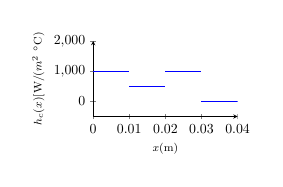
\begin{tikzpicture}[scale=0.5]
	\begin{axis}[
	%/pgf/number format/1000 sep={.},/pgf/number format/use comma,
	axis lines=left,
	xmin = 0,
	xmax = 0.04,
	ymin = -500,
	ymax = 2000,
	restrict y to domain=-500:2000,
	scaled x ticks = false,
	scaled y ticks = false,
	x tick label style={/pgf/number format/fixed},
	y tick label style={/pgf/number format/fixed},
	anchor=east,  
	width=5.25cm,
	height=3.5cm,
	label style={font=\footnotesize},
	xlabel = $x$(m),
	ylabel= $h_c(x)$[W/($\text{m}^2$ \celsius)]]
	\addplot[color=blue,mark=none,smooth, domain=0:0.01] {1000};
	\addplot[color=blue,mark=none,smooth, domain=0.01:0.02] {500};
	\addplot[color=blue,mark=none,smooth, domain=0.02:0.03] {1000};
	\addplot[color=blue,mark=none,smooth, domain=0.03:0.04] {0};
	\end{axis}	
	\end{tikzpicture}	
	\end{minipage}
}%

\newcommand{\legendagraficos}{%
	\caption{$\text{--} \rightarrow \text{Exato}$; $\textcolor{blue}{\ocircle} \rightarrow \sigma = 0.0\celsius$; $\textcolor{red}{\square} \rightarrow \sigma = 0.1\celsius$; $\textcolor{gray}{\triangle} \rightarrow \sigma = 0.5 \celsius$}	
}%


% Let's get started
\begin{document}
\setbeamertemplate{caption}{\raggedright\insertcaption\par}
	
	{
		\usebackgroundtemplate{
			\begin{picture}(210,55)(-5,0)
			\includegraphics[height=0.14\paperwidth,keepaspectratio]{imgs/pem-logo.png}
			\end{picture}%
			\begin{picture}(210,55)(-28,2)
			\includegraphics[height=0.14\paperwidth,keepaspectratio]{imgs/coppe-logo.pdf}
			\end{picture}
		}
		\begin{frame}
			\bigskip\bigskip\bigskip\bigskip
			\titlepage
		\end{frame}
	}
	
\begin{frame}{Agenda}
	\tableofcontents
\end{frame}

\section{Introdução}

\begin{frame}
	\frametitle{Introdução}
	\framesubtitle{Transferência de calor na interface de contato entre dois corpos}
	\begin{figure}[h!b]
		\begin{center}
			\begin{tikzpicture}
			\node at (0, 0)
			{
				\includegraphics[trim=250 642 150 154, clip=true]{imgs/img1.pdf}
			};
			
			\node[scale=0.8] at (0, 0.9) {Sólido 1};
			\node[scale=0.8] at (0, -1.1) {Sólido 2};
			\node[scale=0.8] at (4, 0.3) {Fluido};
			\end{tikzpicture}
		\end{center}
	\end{figure}
\end{frame}

\begin{frame}
	\frametitle{Introdução}
	\framesubtitle{Definição de condutância térmica de contato (CTC)}
	\begin{equation}
	h_c = \frac{q_c}{\Delta T_c}
	\end{equation}
\end{frame}

\begin{frame}
	\frametitle{Introdução}
	\framesubtitle{Aplicações do conceito de condutância térmica de contato}
	\begin{itemize}
		\item Avaliação da qualidade do contato entre corpos materiais
		\begin{itemize}
			\item $q_c = 0 \Rightarrow h_c = 0 \Rightarrow$ isolamento perfeito
			\item $\Delta T_c = 0 \Rightarrow h_c = \infty \Rightarrow$ contato perfeito
		\end{itemize}
		\item Identificação de falhas ou descontinuidades em materiais homogêneos			
	\end{itemize}

\end{frame}
\begin{frame}
	\frametitle{Introdução}
	\framesubtitle{Exemplos de áreas de aplicação}
	\begin{itemize}
		\item Indústria aeroespacial
		\item Microeletrônica
		\item Projeto de trocadores de calor
	\end{itemize}
\end{frame}

%TODO slides de bibliografia apresentando CTC como problema inverso
%TODO apresentar Colaço e Padilha
%TODO apresentar CITT

\section{Problema físico}

\begin{frame}
	\frametitle{Problema físico}
	\framesubtitle{Arranjo físico}
	\begin{figure}[h!b]
		\begin{center}
			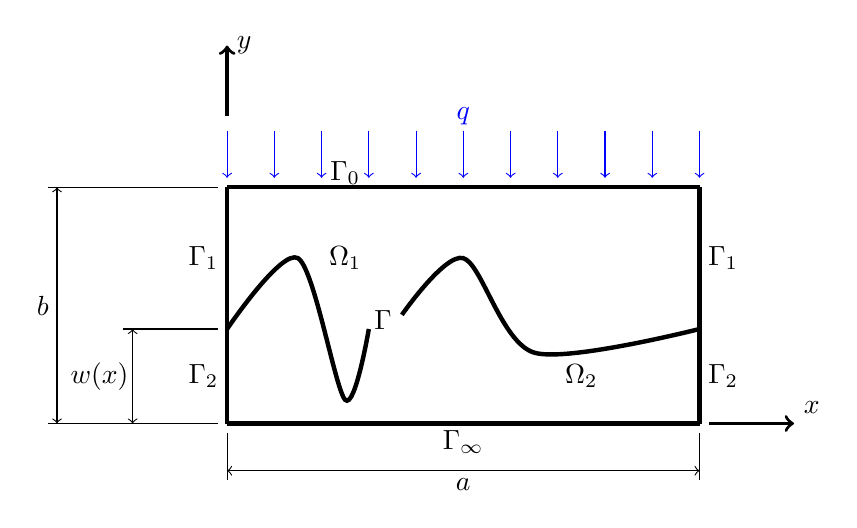
\begin{tikzpicture}[scale=0.6]
			
			\draw [ultra thick] (0, 0) -- (10, 0);
			%\draw [ultra thick] (0, 2) -- (7, 2);
			%\draw [ultra thick] (8, 2) -- (10, 2);
			\draw [ultra thick] plot [smooth] coordinates {(0, 2) (1.5, 3.5) (2.5, 0.5) (3, 2)};
			\draw [ultra thick] plot [smooth] coordinates {(3.7, 2.3) (5, 3.5) (6.5, 1.5) (10, 2)};
			\draw [ultra thick] (0, 5) -- (10, 5);
			\draw [ultra thick] (0, 0) -- (0, 5);
			\draw [ultra thick] (10, 0) -- (10, 5);
			
			\draw (2.5, 3.5) node {$\Omega_1$};
			\draw (7.5, 1) node {$\Omega_2$};	
			\draw (3.3, 2.2) node {$\Gamma$};
			\draw (-0.5, 3.5) node {$\Gamma_1$};
			\draw (-0.5, 1) node {$\Gamma_2$};
			\draw (10.5, 3.5) node {$\Gamma_1$};
			\draw (10.5, 1) node {$\Gamma_2$};
			\draw (5, -0.4) node {$\Gamma_\infty$};
			\draw (2.5, 5.3) node {$\Gamma_0$};
			\draw [blue](5, 6.5) node {$q$};
			\draw (5, -1.3) node {$a$};
			\draw (-3.9, 2.5) node {$b$};
			\draw (-2.7, 1) node {$w(x)$};
			
			\node [above right] at (12, 0) {$x$};
			\node [right] at (0, 8) {$y$};
			
			\draw [->, blue] (0, 6.2) -- (0, 5.2);
			\draw [->, blue] (1, 6.2) -- (1, 5.2);
			\draw [->, blue] (2, 6.2) -- (2, 5.2);
			\draw [->, blue] (3, 6.2) -- (3, 5.2);
			\draw [->, blue] (4, 6.2) -- (4, 5.2);
			\draw [->, blue] (5, 6.2) -- (5, 5.2);
			\draw [->, blue] (6, 6.2) -- (6, 5.2);
			\draw [->, blue] (7, 6.2) -- (7, 5.2);
			\draw [->, blue] (8, 6.2) -- (8, 5.2);
			\draw [->, blue] (9, 6.2) -- (9, 5.2);
			\draw [->, blue] (10, 6.2) -- (10, 5.2);
			
			\draw [->, very thick] (10.2,0) -- (12,0);
			\draw [->, very thick] (0, 6.5) -- (0,8);
			
			\draw [-] (0, -0.2) -- (0, -1.2);
			\draw [-] (10, -0.2) -- (10, -1.2);
			\draw [<->] (0, -1) -- (10, -1);
			
			\draw [-] (-0.2, 0) -- (-3.8, 0);
			\draw [-] (-0.2, 5) -- (-3.8, 5);
			\draw [-] (-0.2, 2) -- (-2.2, 2);
			\draw [<->] (-3.6, 0) -- (-3.6, 5);
			\draw [<->] (-2.0, 0) -- (-2.0, 2);
			
			\end{tikzpicture}
		\end{center}
	\end{figure}
	
	\begin{center}
		\shadowbox{COLAÇO e ALVES (2013); ABREU \textit{et al.} (2016)}
	\end{center}		
\end{frame}

\begin{frame}
	\frametitle{Problema físico}
	\framesubtitle{Formulação}
	\begin{subequations}
		\begin{alignat}{2}
		& \nabla^2 F_{1,j} = 0 \quad\quad\quad\quad\quad && \text{ in } \Omega_1 \label{funcao_F_harm_T1} \\
		& F_{1,j} = \psi_j && \text{ on } \Gamma_0  \label{funcao_F_cc_T1_2} \\
		& \frac{\partial F_{1,j}}{\partial \mathbf{n}_1} = 0 && \text{ on }  \Gamma_1 \label{funcao_F_cc_T1_1} \\ 
		& F_{1,j} = F_{2, j} \quad\quad\quad\quad\quad\quad\quad\quad && \text{ on }  \Gamma \label{funcao_F_cc_grad_T1} \\
		& \nabla^2 F_{2,j} = 0 && \text{ in }  \Omega_2 \label{funcao_F_harm_T2} \\
		& \frac{\partial F_{2,j}}{\partial \mathbf{n}_2} = 0 && \text{ on }  \Gamma_2 \label{funcao_F_cc_T1_3} \\
		& F_{2,j} = 0 && \text{ on }  \Gamma_\infty \label{funcao_F_cc_T1_4} \\
		& k_2\frac{\partial F_{2, j}}{\partial\mathbf{n}_2} = - k_1\frac{\partial F_{1,j}}{\partial\mathbf{n}_1} && \text{ on }  \Gamma \label{funcao_F_cc_T1_5}
		\end{alignat}
	\end{subequations}
\end{frame}

\begin{frame}
	\frametitle{Problema inverso}
	\framesubtitle{Arranjo físico}
	\begin{figure}[h!b]
		\begin{center}
			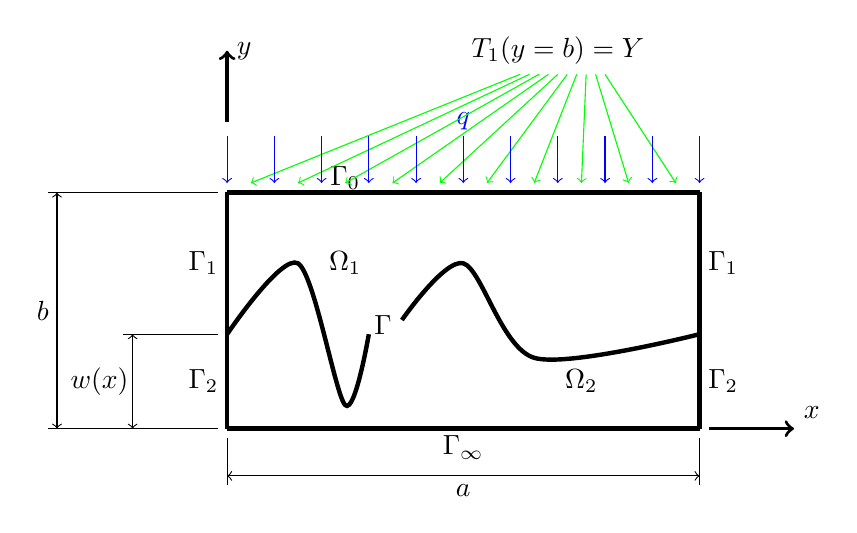
\begin{tikzpicture}[scale=0.6]
			
			\draw [ultra thick] (0, 0) -- (10, 0);
			%\draw [ultra thick] (0, 2) -- (7, 2);
			%\draw [ultra thick] (8, 2) -- (10, 2);
			\draw [ultra thick] plot [smooth] coordinates {(0, 2) (1.5, 3.5) (2.5, 0.5) (3, 2)};
			\draw [ultra thick] plot [smooth] coordinates {(3.7, 2.3) (5, 3.5) (6.5, 1.5) (10, 2)};
			\draw [ultra thick] (0, 5) -- (10, 5);
			\draw [ultra thick] (0, 0) -- (0, 5);
			\draw [ultra thick] (10, 0) -- (10, 5);
			
			\draw (2.5, 3.5) node {$\Omega_1$};
			\draw (7.5, 1) node {$\Omega_2$};	
			\draw (3.3, 2.2) node {$\Gamma$};
			\draw (-0.5, 3.5) node {$\Gamma_1$};
			\draw (-0.5, 1) node {$\Gamma_2$};
			\draw (10.5, 3.5) node {$\Gamma_1$};
			\draw (10.5, 1) node {$\Gamma_2$};
			\draw (5, -0.4) node {$\Gamma_\infty$};
			\draw (2.5, 5.3) node {$\Gamma_0$};
			\draw [blue](5, 6.5) node {$q$};
			\draw (5, -1.3) node {$a$};
			\draw (-3.9, 2.5) node {$b$};
			\draw (-2.7, 1) node {$w(x)$};
			
			\node at (7, 8) {$T_1(y=b) = Y$};
			\draw [->, green] (6.2, 7.5) -- (0.5, 5.2);
			\draw [->, green] (6.4, 7.5) -- (1.5, 5.2);
			\draw [->, green] (6.6, 7.5) -- (2.5, 5.2);
			\draw [->, green] (6.8, 7.5) -- (3.5, 5.2);
			\draw [->, green] (7, 7.5) -- (4.5, 5.2);
			\draw [->, green] (7.2, 7.5) -- (5.5, 5.2);
			\draw [->, green] (7.4, 7.5) -- (6.5, 5.2);
			\draw [->, green] (7.6, 7.5) -- (7.5, 5.2);
			\draw [->, green] (7.8, 7.5) -- (8.5, 5.2);
			\draw [->, green] (8, 7.5) -- (9.5, 5.2);
			
			\node [above right] at (12, 0) {$x$};
			\node [right] at (0, 8) {$y$};
			
			\draw [->, blue] (0, 6.2) -- (0, 5.2);
			\draw [->, blue] (1, 6.2) -- (1, 5.2);
			\draw [->, blue] (2, 6.2) -- (2, 5.2);
			\draw [->, blue] (3, 6.2) -- (3, 5.2);
			\draw [->, blue] (4, 6.2) -- (4, 5.2);
			\draw [->, blue] (5, 6.2) -- (5, 5.2);
			\draw [->, blue] (6, 6.2) -- (6, 5.2);
			\draw [->, blue] (7, 6.2) -- (7, 5.2);
			\draw [->, blue] (8, 6.2) -- (8, 5.2);
			\draw [->, blue] (9, 6.2) -- (9, 5.2);
			\draw [->, blue] (10, 6.2) -- (10, 5.2);
			
			\draw [->, very thick] (10.2,0) -- (12,0);
			\draw [->, very thick] (0, 6.5) -- (0,8);
			
			\draw [-] (0, -0.2) -- (0, -1.2);
			\draw [-] (10, -0.2) -- (10, -1.2);
			\draw [<->] (0, -1) -- (10, -1);
			
			\draw [-] (-0.2, 0) -- (-3.8, 0);
			\draw [-] (-0.2, 5) -- (-3.8, 5);
			\draw [-] (-0.2, 2) -- (-2.2, 2);
			\draw [<->] (-3.6, 0) -- (-3.6, 5);
			\draw [<->] (-2.0, 0) -- (-2.0, 2);
			
			\end{tikzpicture}
		\end{center}
	\end{figure}
\end{frame}

\begin{frame}
	\frametitle{Problema inverso}
	\framesubtitle{Formulação}
	\begin{align*}
	& q_c = -k_1\frac{\partial T_1}{\partial \mathbf{n}_1}\bigg|_\Gamma
	=
	h_c(T_1 - T_2)_\Gamma \\ \\
	& \therefore h_c = \frac{-k_1\displaystyle\frac{\partial T_1}{\partial \mathbf{n}_1}\bigg|_\Gamma}{(T_1 - T_2)_\Gamma}
	\end{align*}
\end{frame}

\begin{frame}
	\frametitle{Funcional de reciprocidade}
	\begin{definition}{}
		\begin{align*}
		\Re(F) = \int_{\Gamma_0}\left[\left(\frac{-q}{k_1}\right)F - Y\frac{\partial F}{\partial\mathbf{n_1}}\right]d\Gamma_0
		\end{align*}
	\end{definition}
	
	\begin{center}
		\shadowbox{COLAÇO e ALVES (2012)}
	\end{center}
	
	\begin{center}
		\shadowbox{ANDRIEUX e BEN ABDA (1993)}
	\end{center}	
\end{frame}

\begin{frame}
	\frametitle{Funcional de reciprocidade}
	
	\begin{corollary}
		\begin{align*}
		k_1\int_{\Gamma_0}\left[\left(\frac{-q}{k_1}\right)\right. & \left.F_1 - Y\frac{\partial F_1}{\partial\mathbf{n_1}}\right]d\Gamma_0
		=\int_\Gamma k_1 \frac{\partial F_1}{\partial\mathbf{n_1}}\left(T_1 - T_2\right)d\Gamma
		\label{identidade_T} \\ \nonumber \\
		k_1\int_{\Gamma_0}\left[\left(\frac{-q}{k_1}\right)\right. & \left.G_1 -  Y\frac{\partial G_1}{\partial\mathbf{n_1}}\right]d\Gamma_0
		= \int_\Gamma -k_1 G_1 \frac{\partial T_1}{\partial\mathbf{n_1}}d\Gamma
		\end{align*}
	\end{corollary}
	
	\begin{center}
		\shadowbox{COLAÇO e ALVES (2012)}
	\end{center}
	
	\begin{alertblock}{}
	Relação entre \textit{as medidas
		do salto de temperatura e de fluxo de calor na interface} $\Gamma$ com \textit{as medidas de temperatura} $Y$ \textit{tomadas na superfície} $\Gamma_0$
	\end{alertblock}
\end{frame}

\begin{frame}
	\frametitle{Espaço linear de funções $L^2(\Gamma)$}
	
	\begin{align*}
		\begin{array}{ll}
			-k_1 \displaystyle \frac{\partial T_1}{\partial\mathbf{n_1}}\bigg|_\Gamma & \in L^2(\Gamma) \\ \\		
			T_1 - T_2|_\Gamma & \in L^2(\Gamma)\\ \\
			k_1 \displaystyle\frac{\partial F}{\partial\mathbf{n_1}}\bigg|_\Gamma & \in L^2(\Gamma) \\ \\
			G|_\Gamma & \in L^2(\Gamma)			
		\end{array}
	\end{align*}
	\pause
	Funções auxiliares:
	\begin{align*}
	& \beta_j \equiv k_1 \frac{\partial F_{1,j}}{\partial\mathbf{n_1}}\bigg|_\Gamma \\ \\
	& \gamma_j \equiv G_{1,j}\big|_\Gamma
	\end{align*}
\end{frame}

\begin{frame}
	\frametitle{Espaço linear de funções $L^2(\Gamma)$}
	\framesubtitle{Produto interno}
	
	\begin{definition}
		\begin{align*}
			\langle f_1, f_2\rangle_{L^2(\Gamma)} = \int_\Gamma f_1(\Gamma) f_2(\Gamma) d\Gamma			
		\end{align*} 
	\end{definition}
	
	\begin{align*}
	& \int_\Gamma k_1 \frac{\partial F_1}{\partial\mathbf{n_1}}\left(T_1 - T_2\right)d\Gamma
	=
	\left\langle \left[T_1 - T_2\right]_\Gamma, \beta_j\right\rangle _{L^2(\Gamma)} \\ \nonumber \\
	&
	\left\langle  -k_1 \frac{\partial T_1}{\partial\mathbf{n_1}}\bigg|_\Gamma, \gamma_j\right\rangle _{L^2(\Gamma)}
	\end{align*} 
\end{frame}

\begin{frame}
	\begin{table}[H]
		\centering
		\caption{Parâmetros usados nos problemas-teste}
		\begin{tabular}{|l|l|}
			\hline
			\textbf{Parâmetro} & \textbf{Valor}  \\ \hline
			$a$       & 0.04 m   \\ \hline
			$b$       & 0.02 m     \\ \hline
			$k_1$     & 54 W/(m \celsius)  \\ \hline
			$k_2$     & 14 W/(m \celsius) \\ \hline
			$q$       & -100,000 W/$\text{m}^2$ \\ \hline
			$h_{max}$       & 1000 W/($\text{m}^2$ \celsius) \\ \hline
		\end{tabular}		
		\label{tabela_params}
	\end{table}
\end{frame}

	
\end{document}